\documentclass[9pt, aspectratio=169, handout]{beamer}

% +==================================================+
% |   ████████╗██╗  ██╗███████╗███╗   ███╗███████╗   |
% |   ╚══██╔══╝██║  ██║██╔════╝████╗ ████║██╔════╝   |
% |      ██║   ███████║█████╗  ██╔████╔██║█████╗     |
% |      ██║   ██╔══██║██╔══╝  ██║╚██╔╝██║██╔══╝     |
% |      ██║   ██║  ██║███████╗██║ ╚═╝ ██║███████╗   |
% |      ╚═╝   ╚═╝  ╚═╝╚══════╝╚═╝     ╚═╝╚══════╝   |
% +==================================================+

\useinnertheme{rectangles}
\useoutertheme{infolines}

\setbeamertemplate{footline}{%
    \leavevmode%
    \rule{\paperwidth}{0.1pt}\vskip0.2pt%
    \hbox{%
        \begin{beamercolorbox}[wd=.2\paperwidth, ht=2.25ex, dp=1ex, center]{author in head/foot}%
            \usebeamerfont{author in head/foot}\insertshortauthor
        \end{beamercolorbox}%
        \begin{beamercolorbox}[wd=.6\paperwidth, ht=2.25ex, dp=1ex, center]{title in head/foot}%
            \usebeamerfont{title in head/foot}\insertshorttitle
        \end{beamercolorbox}%
        \begin{beamercolorbox}[wd=.2\paperwidth, ht=2.25ex, dp=1ex, center]{date in head/foot}%
            \usebeamerfont{date in head/foot}\insertshortdate\hfill\insertframenumber{} / \inserttotalframenumber\hspace*{2ex}
        \end{beamercolorbox}%
    }%
    \vskip0pt%
}
% hrule under the frametitle, see:
% https://tex.stackexchange.com/questions/343517/beamer-full-width-hrule-below-frame-title
\setbeamertemplate{frametitle}{%
    \usebeamerfont{frametitle}\insertframetitle%
    \vphantom{g}%
    \par%
    \makebox[\linewidth][c]{%
        \rule[0.5\baselineskip]{\paperwidth}{0.4pt}%
    }%
}

% \beamertemplatenavigationsymbolsempty % remove navigation bar

\definecolor{grey80}{HTML}{CCCCCC}
\definecolor{grey90}{HTML}{E6E6E6}
\definecolor{grey95}{HTML}{F2F2F2}

\usepackage[svgnames, x11names]{xcolor}
\usecolortheme[named=DarkSlateGrey]{structure}
\setbeamercolor{background canvas}{bg=white}

\setbeamerfont{frametitle}{series=\bfseries}

\let\oldtiny\tiny
\let\oldscriptsize\scriptsize
\let\oldfootnotesize\footnotesize
\let\oldsmall\small
\let\oldnormalsize\normalsize
\let\oldlarge\large
\let\oldLarge\Large
\let\oldLARGE\LARGE
\let\oldhuge\huge
\let\oldHuge\Huge
\renewcommand*{\footnotesize}{\oldfootnotesize\scriptsize}
\renewcommand*{\normalsize}{\oldnormalsize\oldsmall}
\setbeamerfont{frametitle}{size=\oldnormalsize}

% +=================================+
% |   ██████╗ ██╗██████╗ ███████╗   |
% |   ██╔══██╗██║██╔══██╗██╔════╝   |
% |   ██████╔╝██║██████╔╝███████╗   |
% |   ██╔══██╗██║██╔══██╗╚════██║   |
% |   ██████╔╝██║██████╔╝███████║   |
% |   ╚═════╝ ╚═╝╚═════╝ ╚══════╝   |
% +=================================+

% \usepackage[style=nejm,backend=biber]{biblatex}
% \addbibresource{my.bib}
% \renewcommand*{\bibfont}{\footnotesize}

% +==========================================+
% |   ███╗   ███╗ █████╗ ████████╗██╗  ██╗   |
% |   ████╗ ████║██╔══██╗╚══██╔══╝██║  ██║   |
% |   ██╔████╔██║███████║   ██║   ███████║   |
% |   ██║╚██╔╝██║██╔══██║   ██║   ██╔══██║   |
% |   ██║ ╚═╝ ██║██║  ██║   ██║   ██║  ██║   |
% |   ╚═╝     ╚═╝╚═╝  ╚═╝   ╚═╝   ╚═╝  ╚═╝   |
% +==========================================+

\usepackage{amsmath,amssymb,amsfonts}
\usepackage{cancel}
\usepackage{braket}
\usepackage{bm}
\usepackage{siunitx}
\usepackage{feynmf}
\usepackage{cleveref}
\DeclareGraphicsRule{*}{mps}{*}{}

% +===================================================+
% |   ███████╗██╗ ██████╗ ██╗   ██╗██████╗ ███████╗   |
% |   ██╔════╝██║██╔════╝ ██║   ██║██╔══██╗██╔════╝   |
% |   █████╗  ██║██║  ███╗██║   ██║██████╔╝█████╗     |
% |   ██╔══╝  ██║██║   ██║██║   ██║██╔══██╗██╔══╝     |
% |   ██║     ██║╚██████╔╝╚██████╔╝██║  ██║███████╗   |
% |   ╚═╝     ╚═╝ ╚═════╝  ╚═════╝ ╚═╝  ╚═╝╚══════╝   |
% +===================================================+
\usepackage{subcaption}
\usepackage{makecell}
\usepackage{booktabs}

% +===========================================================+
% |    ██████╗██╗  ██╗██╗███╗   ██╗███████╗███████╗███████╗   |
% |   ██╔════╝██║  ██║██║████╗  ██║██╔════╝██╔════╝██╔════╝   |
% |   ██║     ███████║██║██╔██╗ ██║█████╗  ███████╗█████╗     |
% |   ██║     ██╔══██║██║██║╚██╗██║██╔══╝  ╚════██║██╔══╝     |
% |   ╚██████╗██║  ██║██║██║ ╚████║███████╗███████║███████╗   |
% |    ╚═════╝╚═╝  ╚═╝╚═╝╚═╝  ╚═══╝╚══════╝╚══════╝╚══════╝   |
% +===========================================================+

% \usepackage{xeCJK}
% \setCJKmainfont{PingFang SC}

% +====================================+
% |   ███╗   ███╗██╗███████╗ ██████╗   |
% |   ████╗ ████║██║██╔════╝██╔════╝   |
% |   ██╔████╔██║██║███████╗██║        |
% |   ██║╚██╔╝██║██║╚════██║██║        |
% |   ██║ ╚═╝ ██║██║███████║╚██████╗   |
% |   ╚═╝     ╚═╝╚═╝╚══════╝ ╚═════╝   |
% +====================================+

\usepackage{fontawesome5}
\usepackage{twemojis}
\newcommand{\myhl}[1]{\textcolor{DeepPink}{#1}}
\newcommand{\myhlb}[1]{\textcolor{Blue}{#1}}


\title{MAE 131A Discussion Sections\\ Week 8}
\author{Chuanjin Su}
\institute[UCLA MAE]{Mechanical and Aerospace Engineering Department\\
    University of California, Los Angeles}
\date{Nov 22, 2024}

\begin{document}

\begin{frame}
    \titlepage
\end{frame}

\begin{frame}{Problem 1 (10.12 in the book)}
    \begin{columns}
        \column{.6\textwidth}
        \textbf{Problem 1}. The bottom of a copper pan, \SI{150}{mm} in diameter, is maintained at \SI{115}{\celsius} by the heating element of an electric range. Estimate the power required to boil the water in this pan. Determine the evaporation rate. What is the ratio of the surface heat flux to the critical heat flux?
    \end{columns}
\end{frame}

\begin{frame}{Problem 1 Solution}
    \textbf{Solution}. For a temperature difference of \SI{15}{\celsius}, it is safe to assume to undergo nucleate boiling. Using Rohsenow correlation:
    $$
    q'' = \mu_l h_{fg} \left[\frac{g(\rho_l - \rho_v)}{\sigma}\right]^{1/2} \left(\frac{c_{p,l}\Delta T_e}{C_{s,f}h_{fg}\mathrm{Pr}_l^n}\right)^3
    $$
    with $C_{s,f} = 0.0128, n = 1.0$ for water-copper interface. Using the properties $T_{\text{sat}} = \SI{100}{\celsius}, \rho_l = \SI{957.9}{kg/m^3}, \rho_v = \SI{0.5955}{kg/m^3}, c_{p,l} = \SI{4217}{J/kg.K}, \mu_l = \SI{279e-6}{N.s/m^2}, \mathrm{Pr}_l = 1.76, h_{fg} = \SI{2257}{kJ/kg}, \sigma = \SI{58.9e-3}{N/m}$, it can be calculated,
    $$
    q'' = \SI{4.839e5}{W/m^2}
    $$
    thus, the power required is,
    $$
    q_{\text{boil}} = q'' \cdot \frac{\pi D^2}{4} = \SI{8.55}{kW}
    $$
    The maximum heat flux can be determined by,
    $$
    q''_{\text{max}} = 0.149 h_{fg}\rho_v \left[\frac{\sigma g (\rho_l - \rho_v)}{\rho_v^2}\right]^{\frac{1}{4}} = \SI{1.26e6}{W/m^2}
    $$
    therefore, $\frac{q''}{q''_{\text{max}}} = 0.384$.
    \hfill\qedsymbol
\end{frame}

\begin{frame}{Problem 2 (12.41 in the book)}
    \begin{center}
        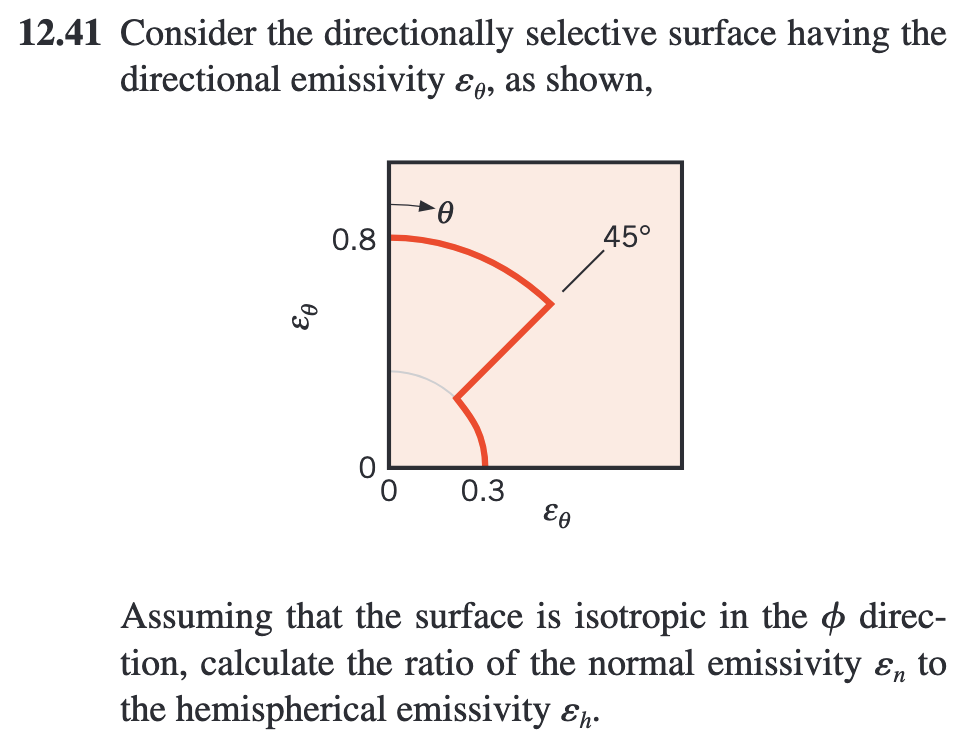
\includegraphics[width=.5\textwidth]{Figures/problem_12.41.png}
    \end{center}
\end{frame}

\begin{frame}{Problem 2 Solution}
    \textbf{Solution}. Normal emissivity $\varepsilon_n = 0.8$ has been given by the problem. However, the hemispherical emissivity $\varepsilon_h$ should be calculated by the integration over the hemisphere,
    \begin{equation*}
        \begin{aligned}
            \varepsilon_h &= 2 \int_0^{\frac{\pi}{2}} \varepsilon_{\theta} \cos\theta \sin\theta d\theta \\
            &= \int_{0}^{\frac{\pi}{4}} 0.3 \sin(2\theta) d\theta + \int_{\frac{\pi}{4}}^{\frac{\pi}{2}} 0.8 \sin(2\theta) d\theta \\
            &= 0.3\times \left[-\frac{1}{2}\cos(2\theta)\right]_0^{\frac{\pi}{4}} + 0.8\times \left[-\frac{1}{2}\cos(2\theta)\right]_{\frac{\pi}{4}}^{\frac{\pi}{2}} \\
            &= 0.15 + 0.4 = 0.55
        \end{aligned}
    \end{equation*}
    Thus $\varepsilon_n / \varepsilon_h = 0.8 / 0.55 = 1.45$.
    \hfill\qedsymbol
\end{frame}

\begin{frame}{Problem 3 (13.6 in the book, \textbf{cross-string} method)}
    \begin{center}
        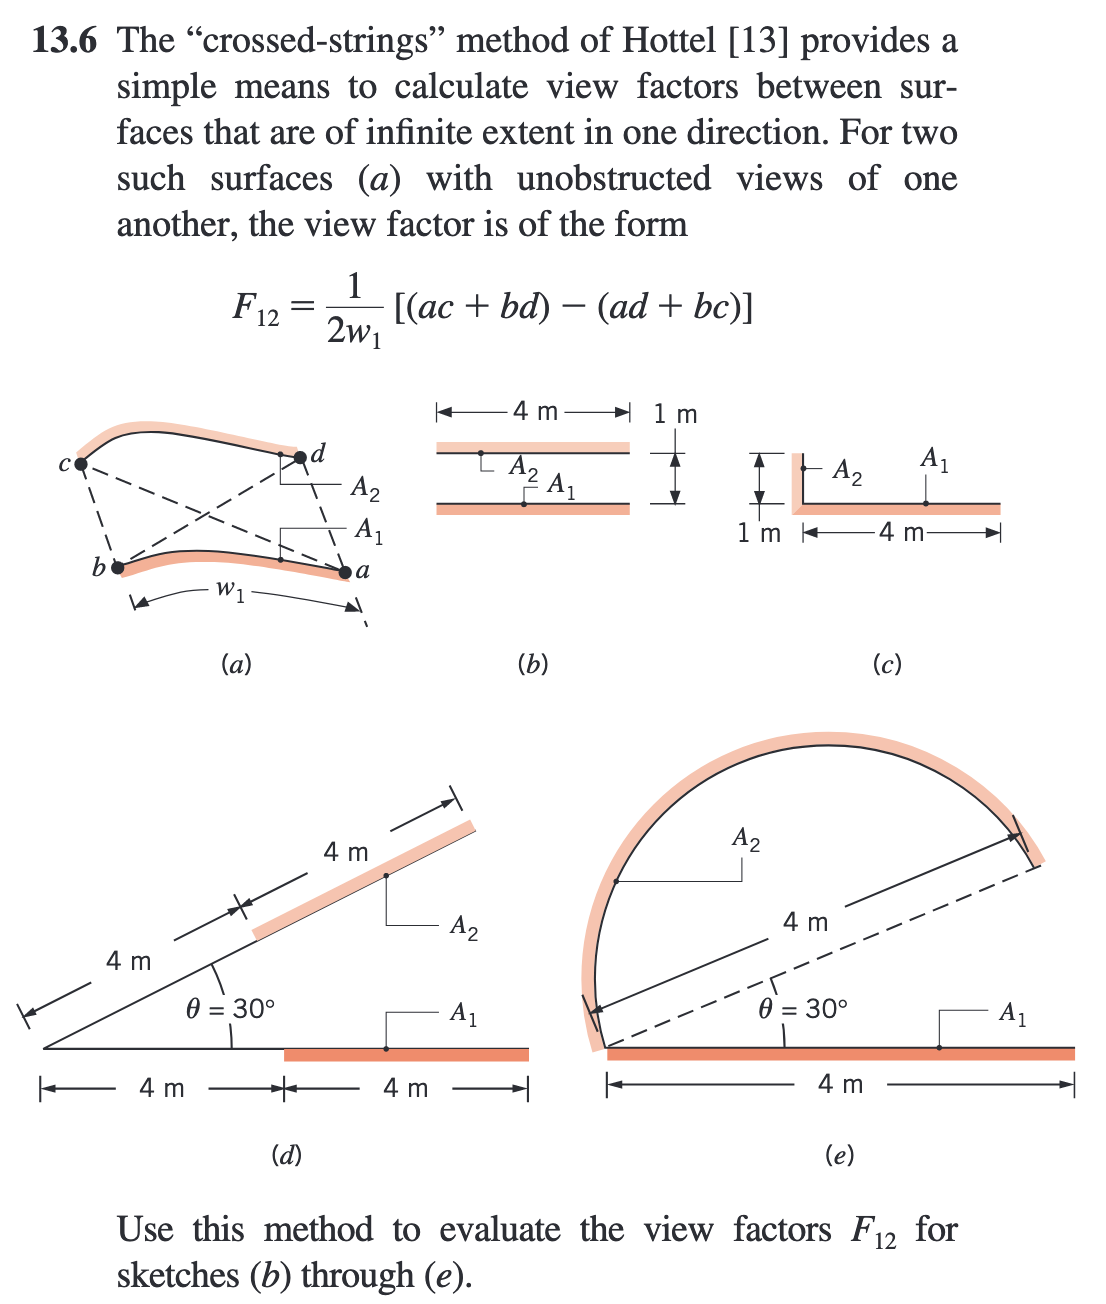
\includegraphics[width=.4\textwidth]{Figures/problem_13.6.png}
    \end{center}
\end{frame}

\begin{frame}{Problem 3 Solution}
    \textbf{Solution}.
    \begin{itemize}
        \item[(b)] it can be seen that $w_1 = \SI{4}{m}$, with $ac = bd = \sqrt{17}, ad = bc = 1$. Thus,
            $$
            F_{12} = \frac{1}{2 \times 4} \left(2\sqrt{17} - 2\right) = 0.7808
            $$
        \item[(c)] $w_1 = \SI{4}{m}$, while $ac = 4, bd = 1, ad = \sqrt{17}, bc = 0$. Therefore,
            $$
            F_{12} = \frac{1}{2 \times 4} \left(4 + 1 - \sqrt{17}\right) = 0.1096
            $$
        \item[(d)] $w_1 = \SI{4}{m}$, with $ac = bd = \sqrt{4^2 + 8^2 - 2\times 4\times 8 \times \cos(30^\circ)} = 4.95725$, $ad = \sqrt{8^2\times 2 - 2 \times 8^2\times \cos (30^\circ)} = 4.14110$, $bc = \sqrt{4^2\times 2 - 2 \times 4^2\times \cos (30^\circ)} = 2.07055$. Thus,
            $$
            F_{12} = \frac{1}{2\times 4} \left(4.95725\times 2 - 4.14110 - 2.07055\right) = 0.4629
            $$
        \item[(e)] $w_1 = \SI{4}{m}$, with $ac = 4, bd = 4, ad = \sqrt{4^2\times 2 - 2 \times 4^2\times \cos (30^\circ)} = 2.07055, bc = 0$. Thus,
            $$
            F_{12} = \frac{1}{2\times 4} \left(4 + 4 - 2.07055\right) = 0.7412
            $$
    \end{itemize}
    \hfill\qedsymbol
\end{frame}

\end{document}
